\chapter{Программная реализация прототипа системы генерации документов на основе шаблонов}
\label{chapter4}

В данном разделе описывается техническая сторона выполнения поставленной задачи. Описан принцип работы исходных текстов, а также процесс реализации механизмов генерации Word-документов. Представлены результаты создания пробного Word-документа 


\section{4.1. Выбор программных средств для реализации системы}

В данном разделе описан процесс выбора инструментальных средств для разработки прототипа генерации Word-документов по шаблону.

В данной работе  было принято решение использовать возможности языка C#. В центре внимания объектно-ориентированного подхода ставятся объекты (абстрактные сущности). Это позволяет разбивать большие задачи на некоторое множество объектов и описывать отношения между ними. В такой модели объекты — это самостоятельные юниты, т. е. объекты способны получать сообщения друг от друга и реагировать на них, регулируя, тем самым, собственное поведение. Программирование в объектно-ориентированном стиле, являющемся частью императивной парадигмы, представляет собой последовательный переход программы из одного состояния в другое.

С# позволяет стартовать разработку быстрее, а это позволяет быстрее получить прототип решения. Скорость разработки на С# на начальных этапах проекта значительно выше по сравнению с С++.

C# спроектирован быть кросплатформенным, однако его развитие не пошло в этом направлении. Поэтому под Windows образовалась достаточно полная .net инфраструктура; на других же платформах равноценной инфраструктуры не появилось.

Программы C# выполняются на платформе .NET Framework, которая интегрирована в Windows и содержит виртуальную общеязыковую среду выполнения (среду CLR) и унифицированный набор библиотек классов. Среда CLR корпорации Майкрософт представляет собой коммерческую реализацию международного стандарта Common Language Infrastructure (CLI), который служит основой для создания сред выполнения и разработки, позволяющих совместно использовать разные языки и библиотеки.

Для работы с объектами Office было принято использовать инструменты пакета Microsoft.Office.Interop, однако также были рассмотрены и использованы функциональные возможности пользовательской библиотеки EasyDox, которая позволяет генерировать документы Word по шаблону, а также содержит пакет Morpher, в котором описаны методы, реализующие склонение по падежам.

\section{4.2. Реализация механизмов генерации Word-файлов.}

В данном разделе описан процесс реализации механизмов генерации Word-файлов выбранным при помощи выбранных инструментальных средств. Приводится информация о тестировании разработанных механизмов и даётся оценка производительности.

Для понимания механизмов работы с объектами Word и Excel, было принято решение в качестве инструмента программной реализации использовать пакет Microsoft Office Interop,  как универсального средства для решения задачи данного типа.

Несмотря на то, что в базе данных уже имеются вариации словесных конструкций в необходимых падежах, в пакете EasyDox.Morpher присутсвуют классы и методы, позволяющие склонять по падежам, имея только форму именительного.

Был получен простейший пользовательский интерфейс, позволяющий выбрать файл базы данных для чтения, а затем извлечь необходимые данные и сгенерировать документ Word по заданному шаблону. 

Для тестирования работоспособности прототипа был построен простейший шаблон страницы отчетности по результатам защиты ВКР и заполнен данными из базы книги Excel. На рис. 4.1 показан результат работы модуля (выделенным цветом обозначаются поля, заполненные программным путем)

 	\begin{figure}
	\caption{Заполнение тестового документа по шаблону}
	\centering
	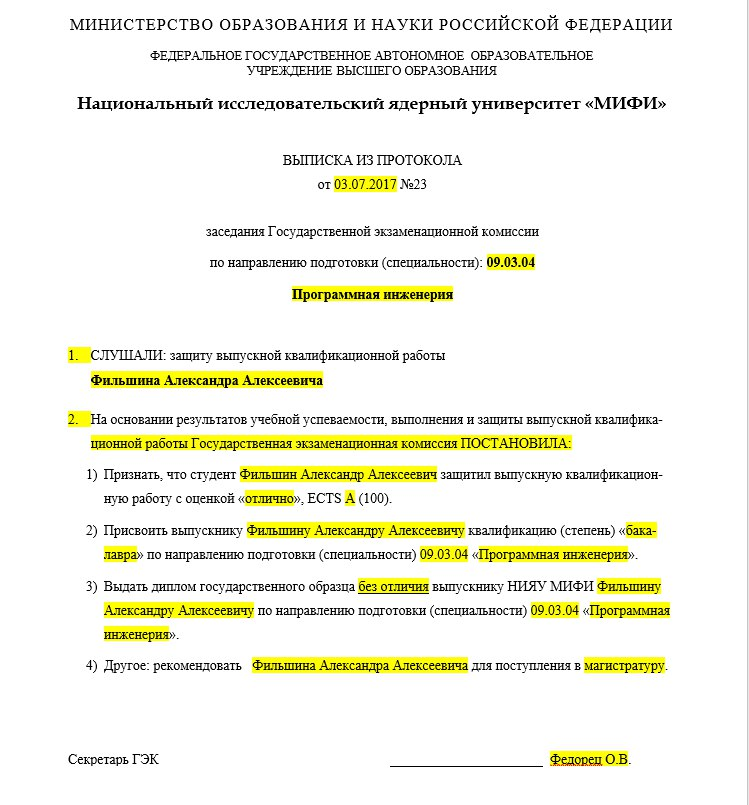
\includegraphics[width=\textwidth]{./screen2.jpg}
\end{figure}







